Navier-Stokes equations is a well known set of PDEs in fluid dynamics to simulate a flow evolution in time. At the University of Orl\'eans, France, the MAPMO laboratory works on a software, called FullSWOF~\footnote{\url{http://www.univ-orleans.fr/mapmo/soft/FullSWOF/}}, which solves the Shallow water equations obtained from the three dimensional Navier-Stokes equations, by averaging on the vertical direction (see e.g.~\cite{Ferrari2004}). Those equations are solved using a two-dimensional Cartesian discretization of the space domain, and a finite volume numerical methods more described in~\cite{CPE:CPE3494}. The MSL program of FullSWOF contains three mesh entities, seven computation domains, fourty-eight data and ninty-eight computations composed of thirty-two stencil kernels and sixty-six local computations.

\subsubsection*{Compiler Evaluation}

The series-parallel tree decomposition $\Gamma_{tsp}$ of this simulation, extracted by the MSC transformation, is composed of seventeen sequence nodes and eighteen parallel nodes. Figure~\ref{fig:freq} represents for a given level of parallelism, \ie the number of tasks to perform concurrently, the number of time this level is observed in the final component assembly. One can notice that the level of task parallelism extracted from the Shallow water equations is limited by two sequential parts in the application (level 1). As a level of sixteen parallel tasks is reached too times, and also five times for the level four, sequential restrictions could be amortized. However, it is rather clear that the task parallelization technique should be used to improve the data parallelism when reaching its limits, but not to use alone. Moreover, as the level of parallelism in the application is heterogenous, the number of threads to launch for task parallelism, and the number of cores to keep for data parallelism is difficult to choose.

\begin{figure}[!h]
 \begin{center}
 \begin{tabular}{c|c|c|c|c|c|c|c|c|}
   level & 1 & 2 & 3 & 4 & 6 & 10 & 12 & 16\\
   \hline
   frequence & 2 & 1 & 3 & 5 & 3 & 1 & 1 & 2\\
 \end{tabular}
\caption{Parallelism level (number of parallel tasks) and the number of times this level appears.}
\label{fig:freq}
 \end{center}
\end{figure}

\begin{figure}[!h]
 \begin{center}
 \begin{tabular}{c|c|c|c|c|}
   step & $\Gamma_{sync}$ & $\Gamma_{dep}$ & $\Gamma_{msp}$ & $\Gamma_{tsp}$\\
   \hline
   time (ms) & 2 & 530 & 8297 & 1133\\
   \hline
   \% & 0.02 & 5.3 & 83.3 & 11.37\\
 \end{tabular}
\caption{Execution times of the MSC transformation steps}
\label{fig:exectime}
 \end{center}
\end{figure}

Figure~\ref{fig:exectime} illustrates the execution time for each step of the MSC transformation for an overall execution time of ten seconds. Execution times have been computed on a laptop with a bi-core Intel Core i5 1,4 GHz, and 8Gb DDR3. 
One can notice that the transformation of $\Gamma_{dep}$ to a minimal series-parallel graph is the longest step of MSC, because of the removal of the forbidden shapes in the graph. Actually, the number of forbidden shapes removed in $\Gamma_{dep}$ is not counted by the algorithm, which applies a general solution (instead of finding each forbidden shape), but it seems that many of them appear. The \emph{N-shape}, represented in Figure~\ref{fig:n} is forbidden in a minimal series-parallel graph as it is not possible to exactly express it using sequences and parallel sections. However, a \emph{N-shape} could perfectly be handled by a dynamic scheduler, for example.
Thus, the fact that many \emph{N-shape} are removed in $\Gamma_{dep}$ shows that the creation of a static shedule of tasks may not be the best solution for complex simulations. It has to be notice, however, that the all computation of $\Gamma_{tsp}$ is still usefull to detect how space loops can be fusionned in $\Gamma_{data}$.

\subsubsection*{Preliminary Performances}
To evaluate performance of the generated component-based parallel structure, we have proceeded as follows. Our current implementation of the MSCAC compiler generates a back-end code using the SkelGIS library. For this reason, our evaluation compare the shallow water equations first parallelized with a pure SkelGIS code (data structures, applicators and interfaces of SkelGIS~\cite{CPE:CPE3494}), and second parallelized with MSL (which uses the SkelGIS data structure). As the SkelGIS library has proved its scalability on the Shallow water equations compared to an MPI parallelization, this performance evaluation should be relevant. 
Moreover, as SkelGIS library handles data parallelization for distributed memory architectures, we have limited for now our evaluations to the fusionned data parallelization of MSCAC (dumped from $\Gamma_{data}$). 

Evaluations have been performed on two clusters of \emph{Grid'5000}~\footnote{\url{https://www.grid5000.fr/mediawiki/index.php/Grid5000:Home}}. Figure~\ref{tab:hard} shows hardware configuration of tohse clusters. On the cluster \emph{Edel} (Grenoble site) have been performed three different experiments, each one described with the size of the Cartesian mesh, and the number of time iterations, as follows: (1) $5k \times 5k$, $500$ iterations; (2) $10k \times 10k$, $500$ iterations; (3) $10k \times 10k$, $2k$ iterations. On the cluster \emph{Paravence} (Rennes sites), the two last experiments have been performed.

\begin{figure}[!h]
\begin{center}
 \begin{tabular}{|c|c|c|}
\hline
    Cluster & \textbf{Edel} & \textbf{Paravance}\\
     \hline         
    Proc. & 2 Intel Xeon E5520 & 2 Intel Xeon E52630v3\\
    & (2.27 GHz) & (2.4 GHz)\\
    Cores/n & 8 & 8\\
    Mem./n & 24 GB & 128 GB\\
    Compiler & OpenMPI & OpenMPI\\
    Network & InfiniBand 40G & 10 Gigabit Ethernet\\
\hline
 \end{tabular}
   \caption{\label{tab:grappe}Hardware of clusters used in the experiments.}
 \end{center}
\end{figure}

%Figure~\ref{fig:times} shows the execution times in seconds as a function of the number of cores. 
Figure~\ref{fig:speedup} illustrates a speedup comparison, using the minimum sequential reference time (which is the MSL sequential time). Finally, Figure~\ref{fig:log2} illustrates the logarithmic scale of execution times as a function of the logarithmic scale of the number of cores.
% \begin{figure}[!h]
%  \begin{center}
%  \begin{tabular}{c|c|c|c|c|c|c}
%    Cores & 8 & 16 & 32 & 64 & 128 & 256\\
%    \hline
%    MSL & 998.10 & 544.86 & 285.73 & 139.8 & 76.45 & 48.05\\
%    \hline
%    SkelGIS & 1324.9 & 638.5 & 371.62 & 197.32 & 117.05 & 64.96\\
%  \end{tabular}
% \caption{Execution times for the shallow water equations using MSL and SkelGIS (in seconds).}
% \label{fig:times}
%  \end{center}
% \end{figure}
\begin{figure*}
\begin{center}
\subfloat[Edel\label{fig:speedup1}]{
\resizebox{4cm}{!}{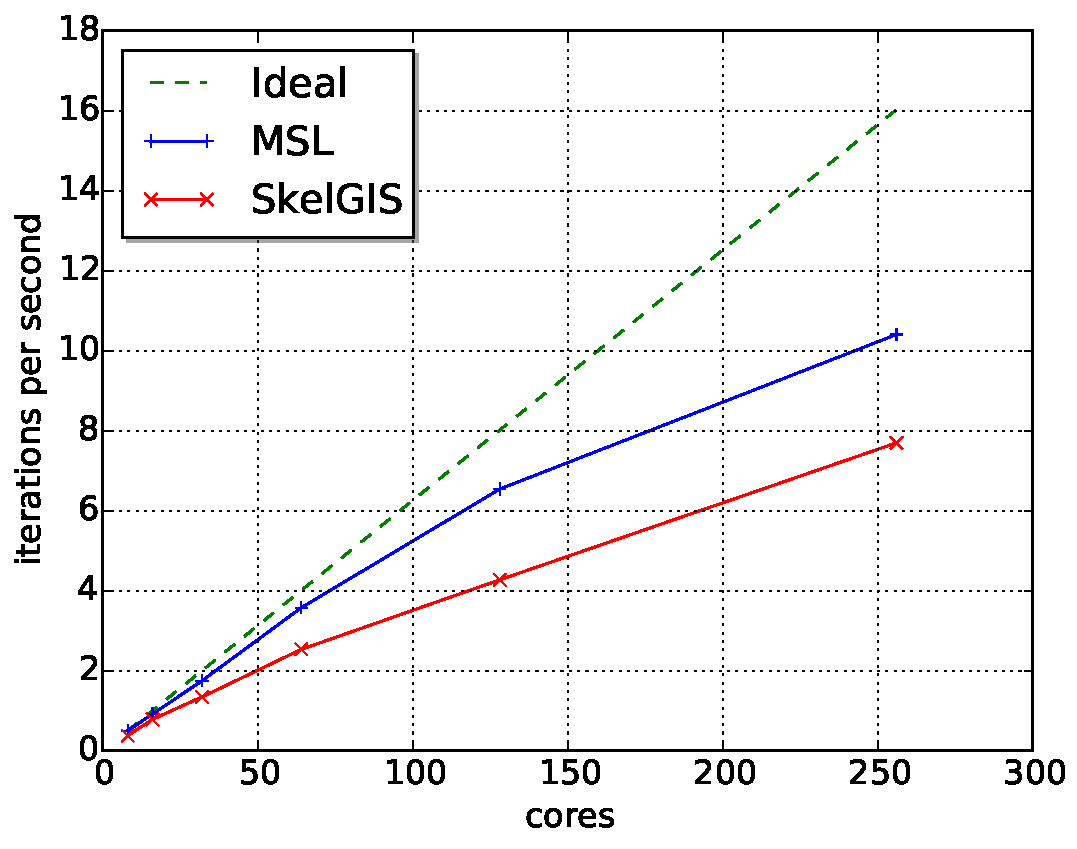
\includegraphics{./images/itpersec_5K_500.pdf}}
}
\hspace{5pt}
\subfloat[Edel\label{fig:log21}]{
\resizebox{4cm}{!}{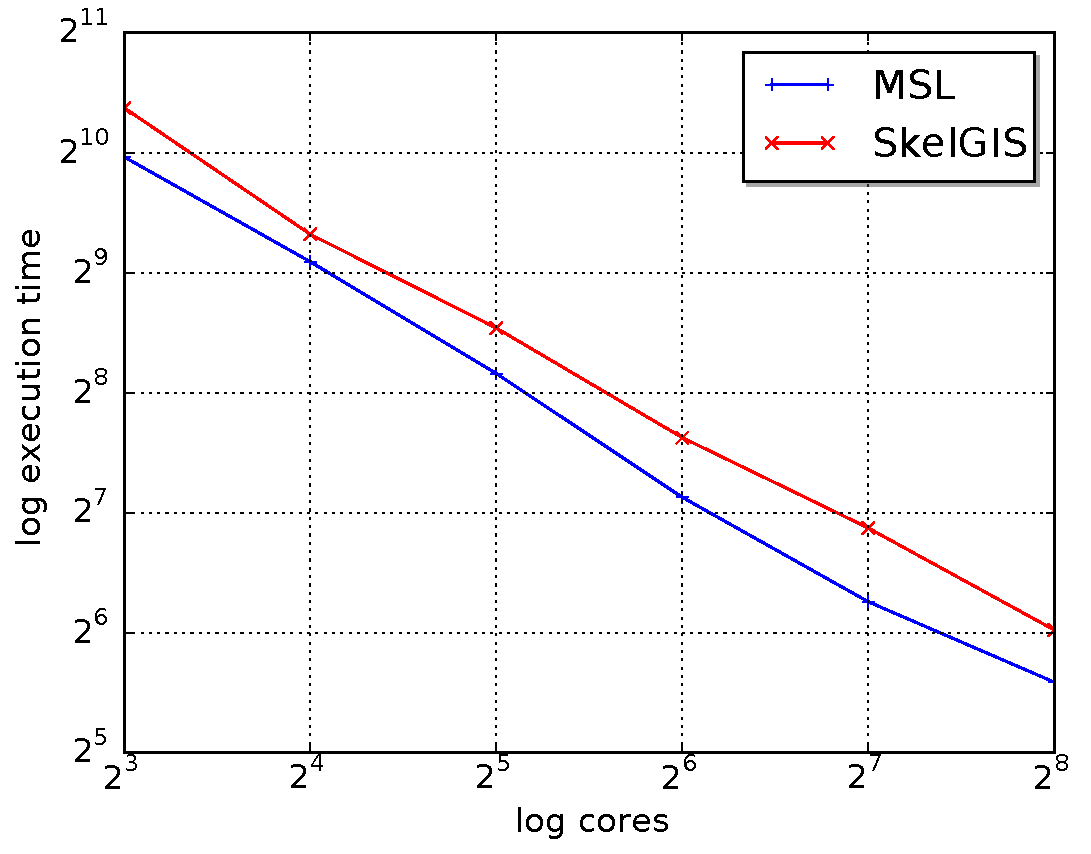
\includegraphics{./images/logtimes_5K_500.pdf}}
}
\hspace{5pt}
\subfloat[Paravance\label{fig:speedup2}]{
\resizebox{4cm}{!}{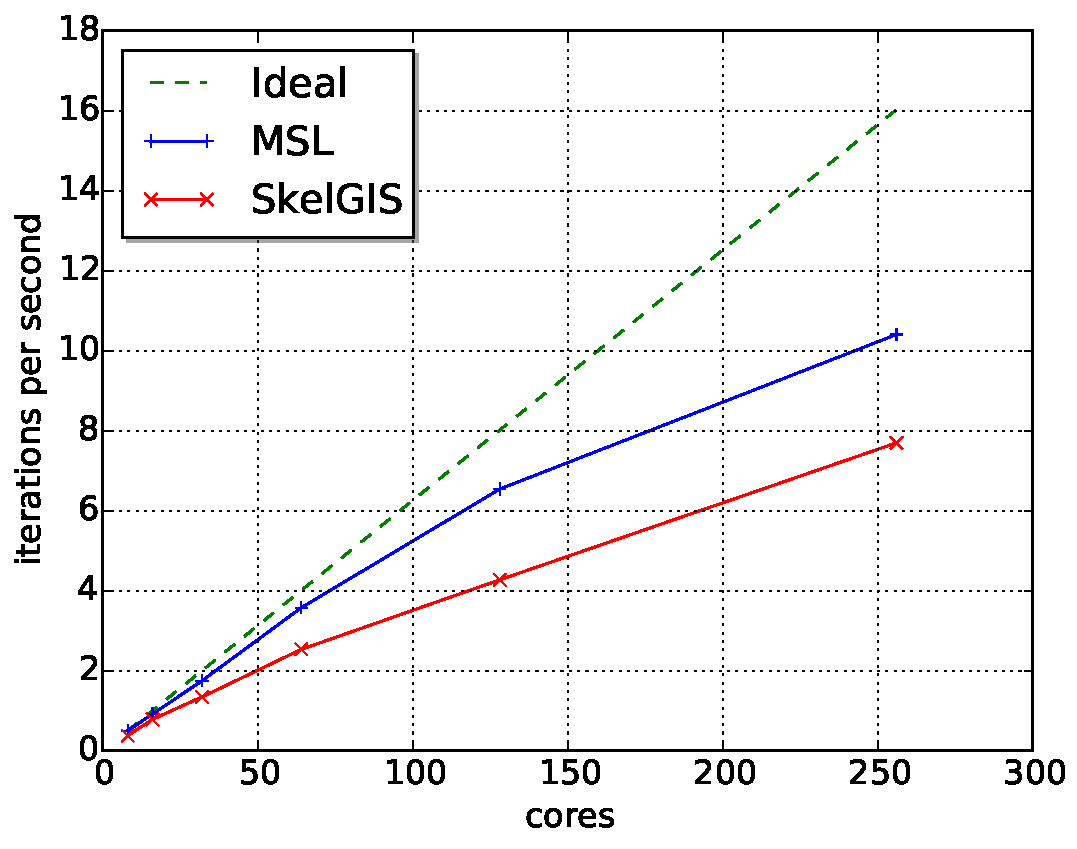
\includegraphics{./images/itpersec_5K_500.pdf}}
}
\hspace{5pt}
\subfloat[Paravance\label{fig:log22}]{
\resizebox{4cm}{!}{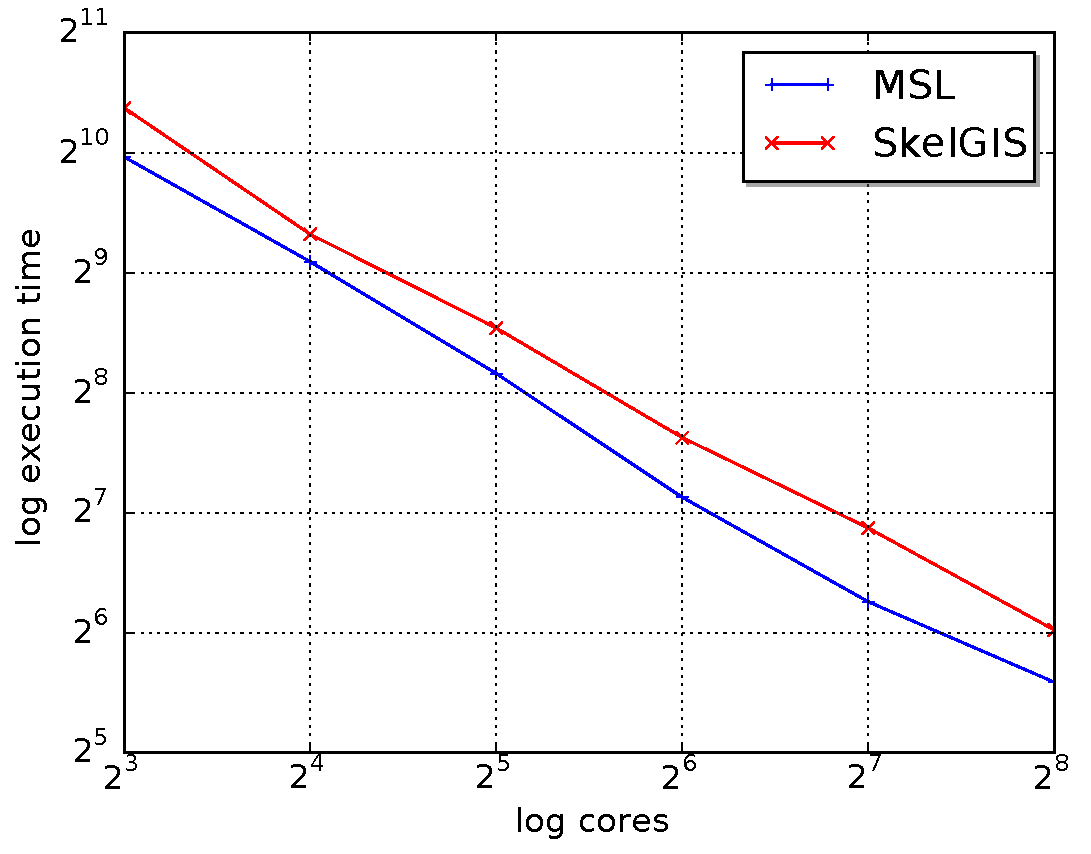
\includegraphics{./images/logtimes_5K_500.pdf}}
}

\subfloat[Edel\label{fig:speedup3}]{
\resizebox{4cm}{!}{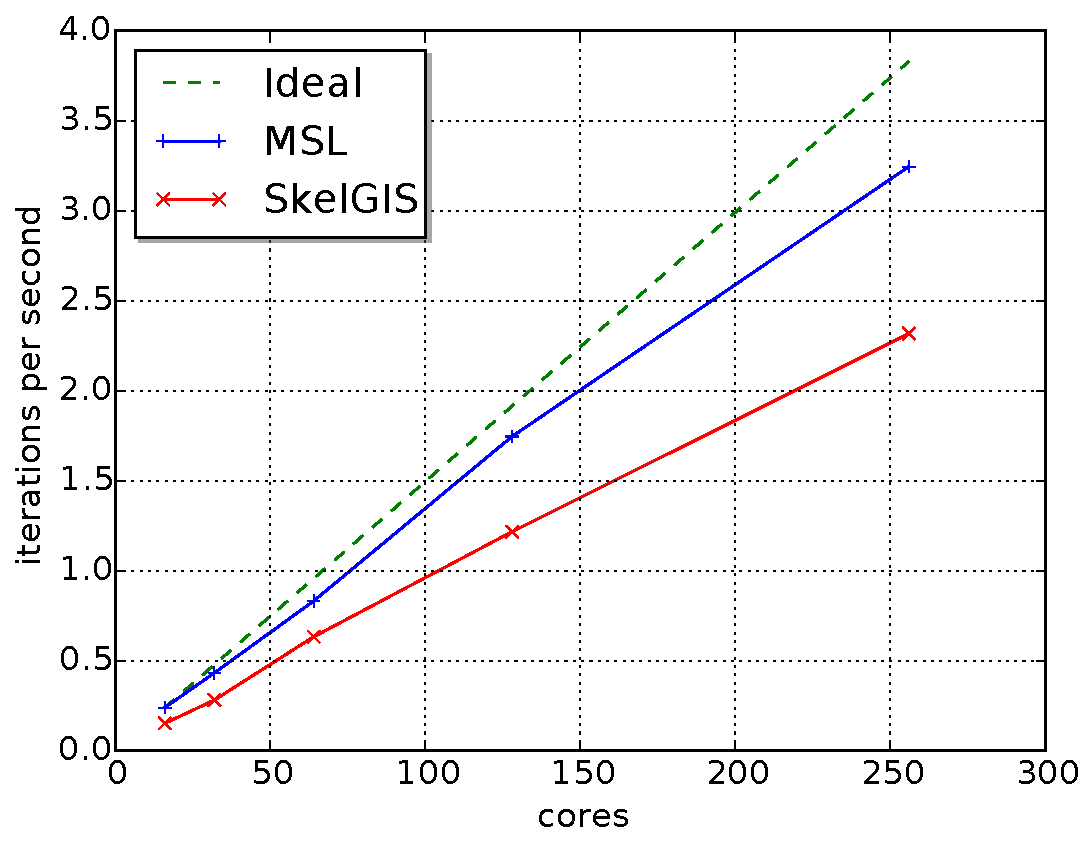
\includegraphics{./images/itpersec_10K_500.pdf}}
}
\hspace{5pt}
\subfloat[Edel\label{fig:log23}]{
\resizebox{4cm}{!}{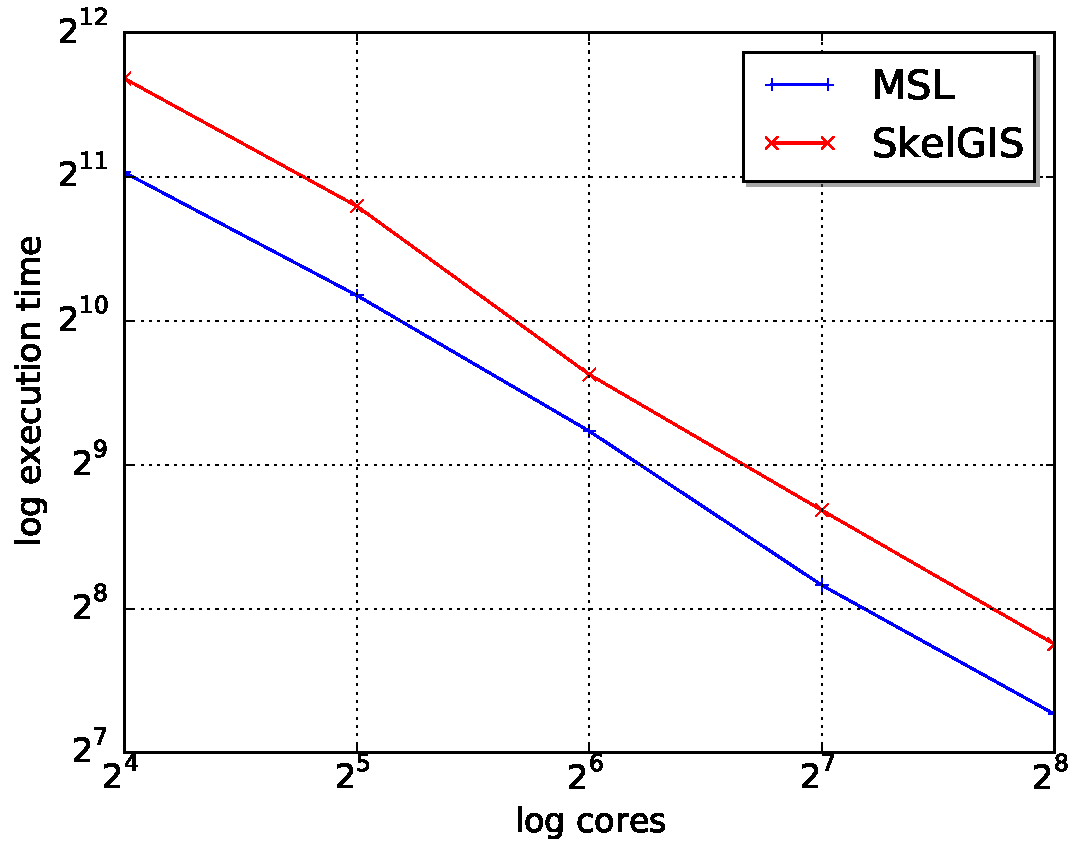
\includegraphics{./images/logtimes_10K_500.pdf}}
}
\hspace{5pt}
\subfloat[Paravance\label{fig:speedup4}]{
\resizebox{4cm}{!}{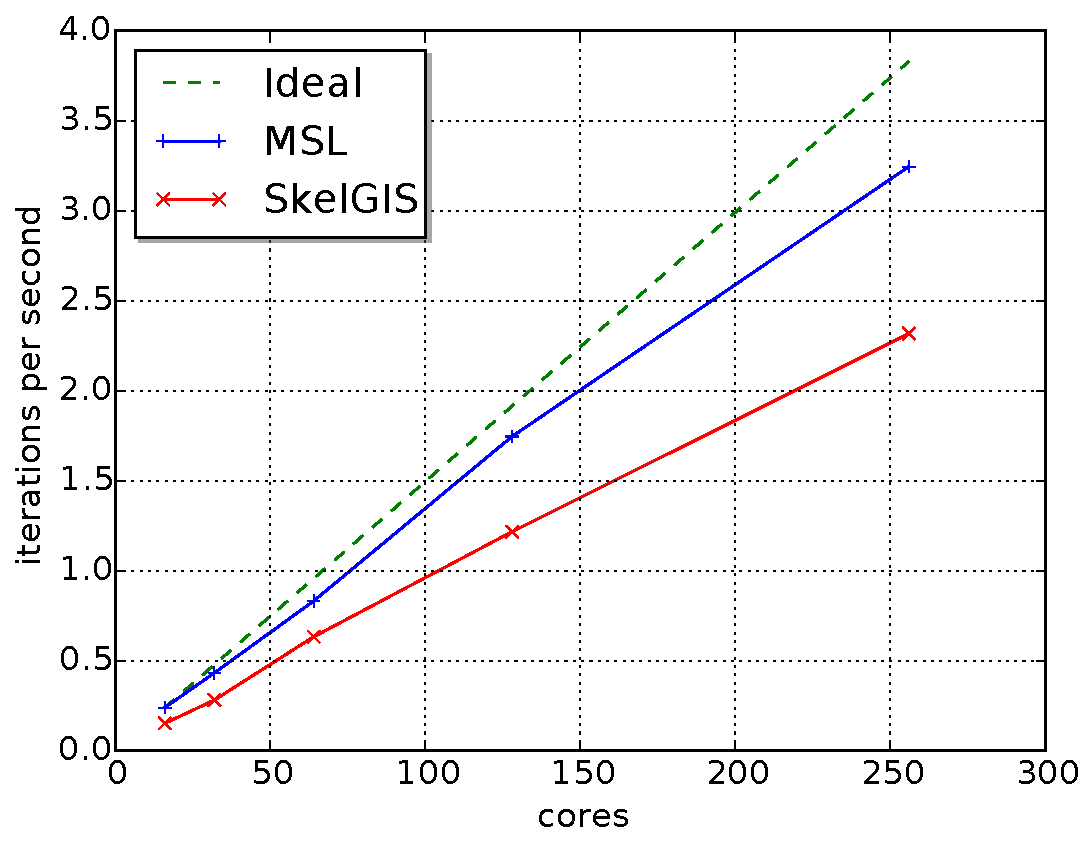
\includegraphics{./images/itpersec_10K_500.pdf}}
}
\hspace{5pt}
\subfloat[Paravance\label{fig:log24}]{
\resizebox{4cm}{!}{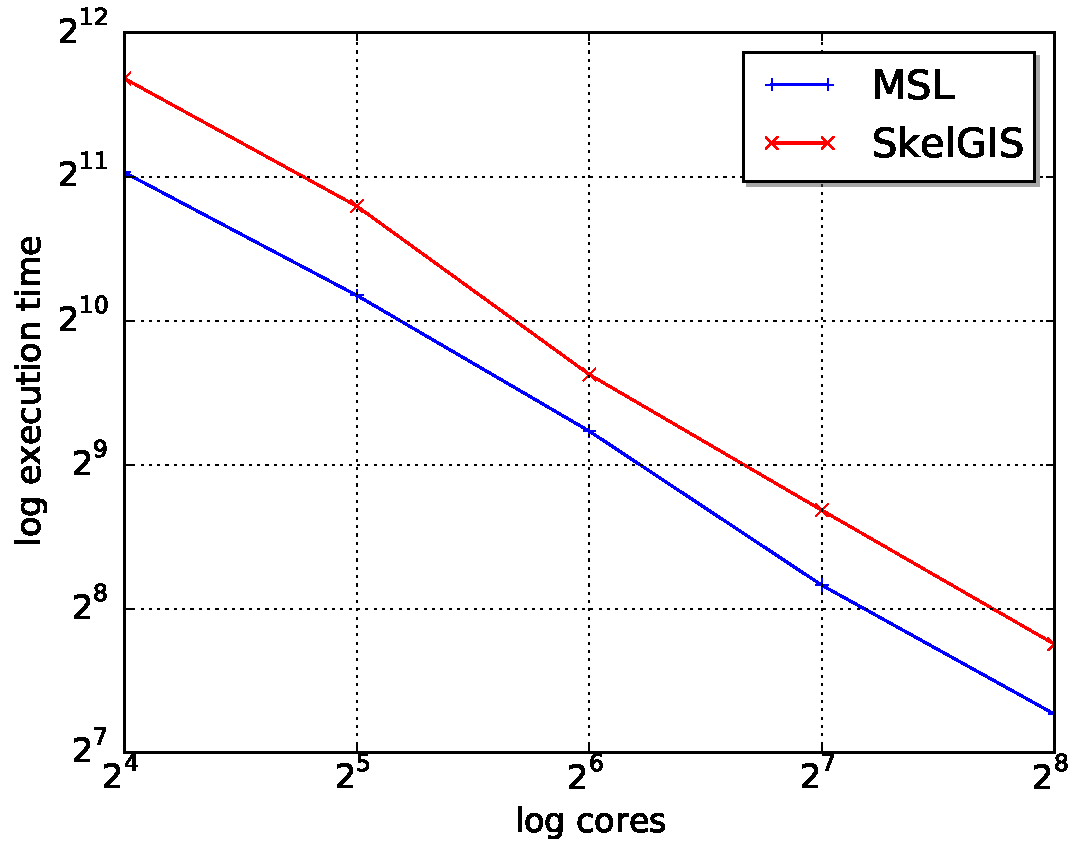
\includegraphics{./images/logtimes_10K_500.pdf}}
}
\end{center}
\caption{(a) Speedup comparison, and (b) logarithmic execution times, both for the Shallow water equations, using pure SkelGIS and MSL with the SkelGIS data structure.}
\label{fig:perfs}
\end{figure*}

One can notice that execution times using MSL, which itself uses the SkelGIS distributed data structures, are improved compared to a pure SkelGIS parallelization. Moreover, the scalability stays close to the scalability of SkelGIS. Thus, using a component-based runtime, performance of the back-end code is still HPC-oriented and does not introduce overheads.

\fix{more figures, more conclusions}
